\chapter{Naive Set Theory and Logic}

Axiomatic set theory is the list of axioms which define sets, on 
which essentially the rest of math is based. Here is given a less 
formal treatment called naive set theory. Taken to its logical 
extreme, it results in contradictions and nonsense. But it serves 
well enough for the purposes of most mathematicians' day-to-day 
work.

Incidentally, there are other solutions to these paradoxes, notably 
type theory and category theory. Homotopy Type Theory (HoTT) is one 
recent formulation which is gaining ground as an alternative 
foundation to mathematics.

%%%%%%%%%%%%%%%%%%%%%%%%%%%%%%%%%%%%%%%%%%%%%%%%%%%%%%%%%%%%%%%%%%

\newpage

\section{Sets}

\subsection{Definition and Examples}\label{sets}

\begin{definition}[Set/Elements of a Set]
	In naive set theory, a \df{set}\index{set} $A$ is a collection 
	of objects. These objects are called the 
	\df{elements}\index{set!element of a} of the set. We write $a 
	\in A$ if $a$ is an element of $A$. We write $a \notin A$ if 
	$a$ is not an element of $A$.
\end{definition}

\begin{example}
	$ $
	\begin{itemize}
		\item The \df{empty set}\index{set!empty set} is the set 
		which contains no elements. We denote the empty set by 
		$\varnothing$.
		
		\item The set of all subsets of a set $A$ is called the 
		\df{power set of $A$}\index{set!power set}, and is 
		denoted by 
		$\ms{P}(A)$.
		
		\item The set of all integers is denoted $\integers$.
	\end{itemize}
\end{example}

We can specify a set in two main ways. The first is to explicitly 
list the elements of the set within curly brackets:
\[
	A = \{ a, b, c \}
\]
The second is to consider as a set all objects which have a certain 
property. For example, we can specify the set $A$ of all people as 
follows:
\[
	A = \{ x \mid x \text{ is a person} \}\,,
\]
which is to be read as ``The set of all $x$ such that $x$ is a 
person.''

This naive view of sets can lead to contradictions since there is 
no restriction on what a set can be. For example, consider 
Russell's paradox: Does the set of all sets which do not contain 
themselves contain itself? Such contradictions are solved in 
axiomatic set theory by restricting what is able to be considered 
a set.

\begin{marginfigure}
	\centering
	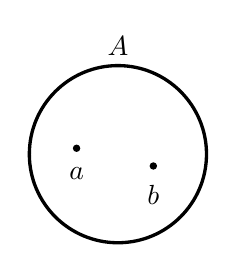
\begin{tikzpicture}[scale=.75]
		\draw[color=black, very thick](0,0) circle (1.5); 
		\node[above] at (0,1.5) {$A$};
		\filldraw (-.7,.1) circle (1.5pt) node[label=below:$a$] 
		{};
		\filldraw (.6,-.2) circle (1.5pt) node[label=below:$b$] 
		{};
	\end{tikzpicture}
	\caption{A set $A$ which contains elements $a$ and 
	$b$.}\label{set}
\end{marginfigure}

Sets are commonly visualized as circles or ovals, as in 
Figure \ref{set}, which depicts a set $A$ containing 
elements $a$ and $b$.

It is common to ``equip'' a set with a structure. For 
example, one could equip a set with a topology, as discussed in 
Section \ref{top space}.

%%%%%%%%%%%%%%%%%%%%%%%%%%%%%%%%%%%%%%%%%%%%%%%%%%%%%%%%%%%%%%%%%%

\newpage

\subsection{Comparing Different Sets}\label{compare sets}

\begin{itemize}
	\item $A$ is a \df{subset}\index{set!subset} of $B$ if every 
	element of $A$ is also an element of $B$, and we write $A 
	\subseteq B$. $A$ is a \df{proper subset} of $B$ if $A$ 
	is a subset of $B$ and $A$ is different from $B$, and we 
	write $A \subsetneq B$. See Figure \ref{subset}.
	
\begin{marginfigure}
	\centering
	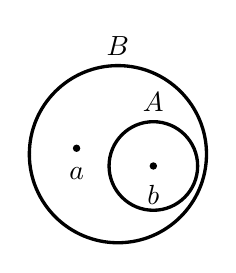
\begin{tikzpicture}[scale=.75]
		\draw[color=black, very thick](0,0) circle (1.5); 
		\node[above] at (0,1.5) {$B$};
		\filldraw (-.7,.1) circle (1.5pt) node[label=below:$a$] 
		{};
		\filldraw (.6,-.2) circle (1.5pt) node[label=below:$b$] 
		{};
		\draw[color=black, very thick](.6,-.2) circle (.75);
		\node[above] at (.6,.55) {$A$};
	\end{tikzpicture}
	\caption{The set $A = \{ b \}$ is a proper subset of the set $B 
	= \{ a,b \}$.}\label{subset}
\end{marginfigure}
	
	\item Two sets are \df{disjoint}\index{set!disjoint sets} 
	if	$A \cap B = \varnothing$.
	
	\item A set is \df{finite}\index{set!finite} if it is 
	empty or if there is a bijection
	\[
	f : A \to \{ 1, 2, \dots, n \}
	\]
	for some positive integer $n$. (See Sec \ref{func props}.) In 
	the former case, we say that $A$ has \df{cardinality} 
	0\index{set!cardinality}; in the latter case, we say that $A$ 
	has \df{cardinality} $n$. If a bijection exists between $A$ and 
	the positive integers, we say that $f$ is \df{countably 
	infinite}. If a set is finite or countably infinite, it is 
	\df{countable}\index{set!countable}. If there exists a 
	bijection between two sets, they have the same cardinality. We 
	denote the cardinality of $A$ by $|A|$. Intuitively, if you can 
	pair up
\end{itemize}

\begin{remark}
	ZXclkJZXlckLxcj...
\end{remark}

%%%%%%%%%%%%%%%%%%%%%%%%%%%%%%%%%%%%%%%%%%%%%%%%%%%%%%%%%%%%%%%%%%

\newpage

\subsection{How to Form New Sets From Given Ones}

\begin{itemize}
	\item Given some sets, we could consider the set to which 
	each of these sets is an element. We refer to this new set as 
	a \df{collection} of sets.
	
	\item Given a collection $\mc{A}$ of sets, the 
	\df{union}\index{set!union of} of the elements of 
	$\mc{A}$ is the set
	\[
	\bigcup_{A \in \mc{A}} A = \{ x \mid x \in A \text{ for 
		at least one } A \in \mc{A} \}\,.
	\]

	\item Given a collection $\mc{A}$ of sets, the 
	\df{intersection}\index{set!intersection of} of the 
	elements of $\mc{A}$ is the set
	\[
	\bigcap_{A \in \mc{A}} A = \{ x \mid x \in A \text{ for 
		every } A \in \mc{A} \}\,.
	\]

\begin{marginfigure}
	\begin{subfigure}{2in}
		\centering
		\begin{venndiagram3sets}[
			tikzoptions={scale=.5,thick},
			shade=pink
		]
			\fillA	\fillB 	\fillC
		\end{venndiagram3sets}
		\caption{Here $\mc{A} = {A, B, C}$ and the shaded region 
			illustrates $\bigcup_{X \in \mc{A}} X$ (or $A \cup B 
			\cup C$).}
	\end{subfigure}
	\begin{subfigure}{2in}
		\centering
		\begin{venndiagram3sets}[
			tikzoptions={scale=.5,thick},
			shade=pink
		]
			\fillACapBCapC
		\end{venndiagram3sets}
		\caption{Here $\mc{A} = {A, B, C}$ and the shaded region 
			illustrates $\bigcap_{X \in \mc{A}} X$ (or $A \cap B 
			\cap C$).}
	\end{subfigure}
	\begin{subfigure}{2in}
		\centering
		\begin{venndiagram2sets}[
			tikzoptions={scale=.5,thick},
			shade=pink
		]
			\fillOnlyA
		\end{venndiagram2sets}
		\caption{The shaded region illustrates $A \setminus B$.}
	\end{subfigure}
	\caption{Visualization of common set operations.}
\end{marginfigure}
	
	\item Given two sets $A$ and $B$, the 
	\df{difference}\index{set!difference of} of $A$ and $B$ is 
	the set
	\[
		A \setminus B = \{ x \mid x \in A \text{ and } x \notin B 
		\}\,.
	\]
	
	\item Let $\{ A_\alpha \}_{\alpha \in J}$ be an indexed family 
	of sets. Let $X = \bigcup_{\alpha \in J} A_\alpha$. We define 
	the \df{cartesian product}\index{set!cartesian product} of this 
	indexed family, denoted by 
	\[
		\prod_{\alpha \in J} A_\alpha\,,
	\]
	to be the set of all $J$-tuples $(x_\alpha)_{\alpha \in J}$ of 
	elements of $X$ such that $x_\alpha \in A_\alpha$ for each 
	$\alpha \in J$.
	
	\item We can also break sets down into constituent parts. The 
	\df{partition}\index{set!partition of} of a set $A$ is a 
	collection 
	of disjoint nonempty subsets of $A$ whose union is all of $A$.
\end{itemize}

\begin{marginfigure}[.25in]
	\begin{subfigure}{2in}
		\centering
		\begin{venndiagram3sets}[
			tikzoptions={scale=.5,thick},
			shade=pink
			]
			\fillACapB 	\fillACapC
		\end{venndiagram3sets}
		\caption{Visualization of the first distributive law.}
	\end{subfigure}
	\begin{subfigure}{2in}
		\centering
		\begin{venndiagram3sets}[
			tikzoptions={scale=.5,thick},
			shade=pink
			]
			\fillOnlyA
		\end{venndiagram3sets}
		\caption{Visualization of the first of DeMorgan's laws.}
	\end{subfigure}
\end{marginfigure}

\begin{theorem}[Laws of Combining Sets]
	$ $
	\begin{itemize}
		\item Set-Theoretic Distributive Laws:
		\begin{align}
			A \cap (B \cup C) &= (A \cap B) \cup (A \cap C)\,; \\
			A \cup (B \cap C) &= (A \cup B) \cap (A \cup C)\,.
		\end{align}
	
		\item DeMorgan's Laws:
		\begin{align}
			A \setminus (B \cup C)
				&= (A \setminus B) \cap (A \setminus C)\,; \\
			A \setminus (B \cap C)
				&= (A \setminus B) \cup (A \setminus C)\,.
		\end{align}
	\end{itemize}
\end{theorem}

%%%%%%%%%%%%%%%%%%%%%%%%%%%%%%%%%%%%%%%%%%%%%%%%%%%%%%%%%%%%%%%%%%
%%%%%%%%%%%%%%%%%%%%%%%%%%%%%%%%%%%%%%%%%%%%%%%%%%%%%%%%%%%%%%%%%%

\newpage

\section{Functions}

\subsection{Definition and Examples}

\begin{definition}
	$ $
	\begin{itemize}
		\item A \df{rule of assignment}\index{function!rule of 
		assignment} 
		is a subset $r$ of the cartesian product $C \times D$ of 
		two sets such that
		\[
			[(c,d) \in r \text{ and } (c,d') \in r] \Ra [d=d']\,.
		\]
		The \df{domain}\index{function!domain} and \df{image 
		set}\index{function!image set} of $r$ are defined as
		\begin{align}
			\domain r &= \{ c \mid \text{there exists } d \in D
				\text{ such that } (c,d) \in r \}\,, \\
			\image r &= \{ d \mid \text{there exists } c \in C 
			\text{ such that } (c,d) \in r \}\,.
		\end{align}
		
		\item A \df{function}\index{function} $f$ is a rule of 
		assignment $r$, together with a set $B$ that contains the 
		image set of $r$. The domain $A$ of the rule $r$ is also 
		called the \df{domain} of the function $f$; the image set 
		of $r$ is also called the \df{image set} of $f$; and the 
		set $B$ is called the 
		\df{codomain}\index{function!codomain} of $f$. We 
		write $f : A \to B$ and say ``$f$ is a function from $A$ 
		to $B$''
		
		\item If $f: A \to B$ and if $a$ is an element of $A$, we 
		denote by $f(a)$ the unique element of $B$ such that $(a, 
		f(a)) \in r$; it is called the 
		\df{value}\index{function!value of element} of $f$ at 
		$a$, or the 
		\df{image}\index{function!image of element} of $a$ 
		under $f$. We also write $a \mapsto b$.
		
		\item Let $f : A \to B$. If $A_0$ is a subset of $A$, we 
		denote by $f(A_0)$ the set $f(A_0) = \{ b \mid b = f(a) 
		\text{ for at least one } a \in A_0 \}$. This set is 
		called the \df{image}\index{function!image of subset} 
		of $A_0$ under $f$. 
		
		\item If $B_0$ is a subset of $B$, we denote by 
		$f^{-1}(B_0)$ the set $f^{-1}(B_0) = \{ a \mid f(a) \in B_0 
		\}.$ This set is called the 
		\df{preimage}\index{function!preimage} of $B_0$ under $f$. The preimage of a single-element set, say $\{ b \}$, under $f$ is called the \df{fiber}\index{function!fiber} of $f$ over $b$.
	\end{itemize}
\end{definition}

\begin{marginfigure}
	\centering
	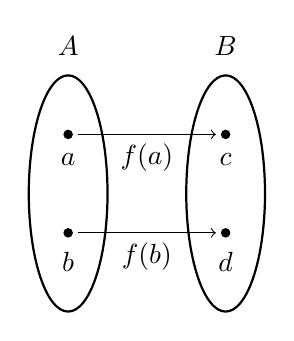
\begin{tikzpicture}
	\draw[thick] (0,0) ellipse (.5 and 1.5);
	\node[label=$A$] at (0,1.5) (A) {};
	\filldraw (0,.75) circle (1.5pt) node[label=below:$a$] (a) {};
	\filldraw (0,-.5) circle (1.5pt) node[label=below:$b$] (b) {};
	
	\draw[thick] (2,0) ellipse (.5 and 1.5);
	\node[label=$B$] at (2,1.5) (B) {};
	\filldraw (2,.75) circle (1.5pt) node[label=below:$c$] (c) {};
	\filldraw (2,-.5) circle (1.5pt) node[label=below:$d$] (d) {};
	
	\draw[->] (a) -- (c) node[midway,below] {$f(a)$};
	\draw[->] (b) -- (d) node[midway,below] {$f(b)$};
	\end{tikzpicture}
	\caption{A function $f$ between the sets $A$ and 
		$B$.}\label{function}
\end{marginfigure}

Intuitively, a function is a mapping from one set to another. 
Functions are commonly visualized as arrows between the elements 
of sets, as in Figure \ref{function}.

%%%%%%%%%%%%%%%%%%%%%%%%%%%%%%%%%%%%%%%%%%%%%%%%%%%%%%%%%%%%%%%%%%

\subsection{How to Form New Functions From Given Ones}

\begin{itemize}
	\item If $f : A \to B$ and if $A_0$ is a subset of $A$, 
	we define the \df{restriction}\index{function!restriction of} 
	of $f$ to $A_0$ to be the function mapping $A_0$ into $B$ 
	whose rule is $\{ (a,f(a)) \mid a \in A_0 \}$. It is denoted 
	by $f|A_0$, and we say ``$f$ restricted to $A_0$.''
	
	\item Given functions $f : A \to B$ and $g : B \to C$, we 
	can define the \df{composite}\index{function!composite} $g 
	\circ 
	f$ (read ``$g$ after $f$'') of $f$ and $g$ as the 
	function 
	$g \circ f : A \to C$ to be the function whose rule is
	\[
	\{ (a,c) \mid \text{For some } b \in B, f(a) = b \text{ 
		and } g(b) = c \}\,.
	\]
	
	\item If $f : A \to B$, then $f$ has a \df{left inverse}\index{function!left inverse} if there is a function $g : B \to A$ such that $g \circ f : A \to A$ is the identity map on $A$, i.e., $(g \circ f)(a) = a$, for all $a \in A$. $f$ has a \df{right inverse}\index{function!left inverse} if there is a function $h : B \to A$ such that $f \circ h : B \to B$ is the identity map on $B$.
	
	\item If $f$ is bijective, there exists a function 
	$f^{-1}$ called the \df{inverse}\index{function!inverse} of 
	$f$ 
	defined by letting $f^{-1}(b)$ be the unique $a$ such 
	that $f(a) = b$.
\end{itemize}

%%%%%%%%%%%%%%%%%%%%%%%%%%%%%%%%%%%%%%%%%%%%%%%%%%%%%%%%%%%%%%%%%%

\subsection{Properties a Function Can Have}\label{func props}
\begin{itemize}
	\item A function $f : A \to B$ is 
	\df{injective}\index{function!injective} (or 
	\df{one-to-one}\index{function!one-to-one}) if
	\[
		[f(a) = f(a')] \Ra [a = a']\,,
	\]
	and \df{surjective}\index{function!surjective} (or 
	\df{onto}\index{function!onto}) if 
	\[
		[b \in B] \Ra [b = f(a) \text{ for at least one } a 
		\in A]\,.
	\]
	If $f$ is both injective and surjective, it is said to be 
	\df{bijective}\index{function!bijective} (or is called a 
	\df{one-to-one correspondence}\index{function!one-to-one 
	correspondence}).
\end{itemize}

\begin{marginfigure}
\begin{subfigure}{2in}
	\centering
	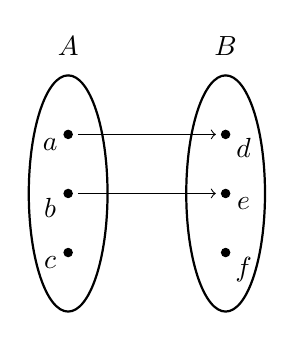
\begin{tikzpicture}
	\draw[thick] (0,0) ellipse (.5 and 1.5);
	\node[label=$A$] at (0,1.5) (A) {};
	\filldraw (0,.75) circle (1.5pt) 
	node[label={[xshift=-6.5pt,yshift=5.5pt]below:$a$}] (a) {};
	\filldraw (0,0) circle (1.5pt) 
	node[label={[xshift=-6.5pt,yshift=5.5pt]below:$b$}] (b) {};;
	\filldraw (0,-.75) circle (1.5pt) 
	node[label={[xshift=-6.5pt,yshift=5.5pt]below:$c$}] (c) {};
	
	\draw[thick] (2,0) ellipse (.5 and 1.5);
	\node[label=$B$] at (2,1.5) (B) {};
	\filldraw (2,.75) circle (1.5pt) 
	node[label={[xshift=6.5pt,yshift=5.5pt]below:$d$}] (d) {};
	\filldraw (2,0) circle (1.5pt) 
	node[label={[xshift=6.5pt,yshift=5.5pt]below:$e$}] (e) {};
	\filldraw (2,-.75) circle (1.5pt) 
	node[label={[xshift=6.5pt,yshift=5.5pt]below:$f$}] (f) {};
	
	\draw[->] (a) -- (d);
	\draw[->] (b) -- (e);
	\end{tikzpicture}
	\caption{This function is injective but not 
	surjective.}\label{inj function}
\end{subfigure}
\begin{subfigure}{2in}
	\centering
	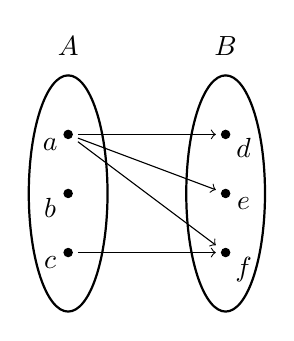
\begin{tikzpicture}
	\draw[thick] (0,0) ellipse (.5 and 1.5);
	\node[label=$A$] at (0,1.5) (A) {};
	\filldraw (0,.75) circle (1.5pt) 
	node[label={[xshift=-6.5pt,yshift=5.5pt]below:$a$}] (a) {};
	\filldraw (0,0) circle (1.5pt) 
	node[label={[xshift=-6.5pt,yshift=5.5pt]below:$b$}] (b) {};;
	\filldraw (0,-.75) circle (1.5pt) 
	node[label={[xshift=-6.5pt,yshift=5.5pt]below:$c$}] (c) {};
	
	\draw[thick] (2,0) ellipse (.5 and 1.5);
	\node[label=$B$] at (2,1.5) (B) {};
	\filldraw (2,.75) circle (1.5pt) 
	node[label={[xshift=6.5pt,yshift=5.5pt]below:$d$}] (d) {};
	\filldraw (2,0) circle (1.5pt) 
	node[label={[xshift=6.5pt,yshift=5.5pt]below:$e$}] (e) {};
	\filldraw (2,-.75) circle (1.5pt) 
	node[label={[xshift=6.5pt,yshift=5.5pt]below:$f$}] (f) {};
	
	\draw[->] (a) -- (d);
	\draw[->] (a) -- (e);
	\draw[->] (a) -- (f);
	\draw[->] (c) -- (f);
	\end{tikzpicture}
	\caption{This function is surjective but not 
	injective.}\label{surj function}
\end{subfigure}
\begin{subfigure}{2in}
	\centering
	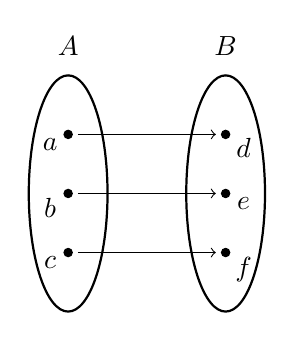
\begin{tikzpicture}
	\draw[thick] (0,0) ellipse (.5 and 1.5);
	\node[label=$A$] at (0,1.5) (A) {};
	\filldraw (0,.75) circle (1.5pt) 
	node[label={[xshift=-6.5pt,yshift=5.5pt]below:$a$}] (a) {};
	\filldraw (0,0) circle (1.5pt) 
	node[label={[xshift=-6.5pt,yshift=5.5pt]below:$b$}] (b) {};;
	\filldraw (0,-.75) circle (1.5pt) 
	node[label={[xshift=-6.5pt,yshift=5.5pt]below:$c$}] (c) {};
	
	\draw[thick] (2,0) ellipse (.5 and 1.5);
	\node[label=$B$] at (2,1.5) (B) {};
	\filldraw (2,.75) circle (1.5pt) 
	node[label={[xshift=6.5pt,yshift=5.5pt]below:$d$}] (d) {};
	\filldraw (2,0) circle (1.5pt) 
	node[label={[xshift=6.5pt,yshift=5.5pt]below:$e$}] (e) {};
	\filldraw (2,-.75) circle (1.5pt) 
	node[label={[xshift=6.5pt,yshift=5.5pt]below:$f$}] (f) {};
	
	\draw[->] (a) -- (d);
	\draw[->] (b) -- (e);
	\draw[->] (c) -- (f);
	\end{tikzpicture}
	\caption{This function is bijective.}\label{bij function}
\end{subfigure}
\caption{Visualizations of injective, surjective, and bijective 
functions.}\label{function examples}
\end{marginfigure}

The basic idea is that if we can find a bijective function 
between two sets, then they are the same ``size'' or 
``cardinality.'' (See Section \ref{compare sets}.)
These properties are illustrated in Figure \ref{function 
examples}. 

The following lemma comes in handy for showing that a given 
function is bijective

\begin{lemma}
	Let $f : A \to B$. If there are functions $g : B \to A$ and 
	$h : B \to A$ such that $g(f(a)) = a$ for every $a$ in $A$ 
	and $f(h(b)) = b$ for every $b$ in $B$, then $f$ is bijective 
	and $g = h = f^{-1}$.
\end{lemma}

\begin{example}
	A \df{permutation}\index{function!permutation} of a set $A$ is simply a bijection from $A$ to itself.
\end{example}

%%%%%%%%%%%%%%%%%%%%%%%%%%%%%%%%%%%%%%%%%%%%%%%%%%%%%%%%%%%%%%%%%%
%%%%%%%%%%%%%%%%%%%%%%%%%%%%%%%%%%%%%%%%%%%%%%%%%%%%%%%%%%%%%%%%%%

\newpage

\section{Relations}

\subsection{Definition and Examples}

\begin{definition}[Relation]
	A \df{binary relation}\index{binary relation} on a set $A$ is a subset $C$ of the cartesian product $A \times A$. We use the notation $xCy$ to mean the same thing as $(x,y) \in C$, and we say ``$x$ is in the relation $C$ to $y$.''
\end{definition}

Remark: This is weaker than a rule of assignment in the sense 
that a given element is allowed to be assigned to more than one 
value of the second set. A function $f:A \to A$ is a special case 
of a relation. Note that both sets are always the same 
in the case of a relation.

For a given relation $C$ on the set $A$, 
\begin{itemize}
	\item A relation is \df{reflexive}\index{binary relation!reflexive} 
	if $xCx$ for every $x$ in $A$.
	
	\item A relation is \df{symmetric}\index{binary relation!symmetric} 
	if $xCy$ implies $yCx$.
	
	\item A relation is 
	\df{transitive}\index{binary relation!transitive} if $xCy$ and $yCz$ 
	together implies $xCz$.
	
	\item A relation is 
	\df{comparable}\index{binary relation!comparable} if for every $x$ 
	and $y$ in $A$ for which $x \neq y$, either $xCy$ or $yCx$.
	
	\item A relation is 
	\df{nonreflexive}\index{binary relation!nonreflexive} if for no $x$ 
	in $A$ does the relation $xCx$ hold.
\end{itemize}

%%%%%%%%%%%%%%%%%%%%%%%%%%%%%%%%%%%%%%%%%%%%%%%%%%%%%%%%%%%%%%%%%%

\subsection{Equivalence Relations}\label{eq 
relation properties}

\begin{definition}[Equivalence Relation]
	An \df{equivalence relation}\index{binary relation!equivalence 
	relation} on a 
	set $A$ is a relation $C$ on $A$ which is reflexive, 
	symmetric, and transitive. We often use $\sim$ for an 
	equivalence relation instead of $C$.
\end{definition}

\begin{itemize}
	\item Given an equivalence relation $\sim$ on a set $A$ and 
	an element $x$ of $A$, we define the \df{equivalence 
	class}\index{binary relation!equivalence class} determined by $x$ as
	\[
		\{ y \mid y \sim x \}\,.
	\]
	If $C$ is an equivalence class, any element of $C$ is called a \df{representative}\index{binary relation!representative of an equivalence class} of the class $C$.
	Two equivalent classes are either disjoint or equal, and the 
	collection of equivalence classes of a set $A$ partition $A$.
\end{itemize}

%%%%%%%%%%%%%%%%%%%%%%%%%%%%%%%%%%%%%%%%%%%%%%%%%%%%%%%%%%%%%%%%%%

\subsection{Order Relations}

\begin{definition}[Order Relation]
	An \df{order relation}\index{binary relation!order relation} on a 
	set $A$ is a relation $C$ on $A$ which is comparable, 
	nonreflexive, and transitive. We often use $<$ for an 
	order relation instead of $C$.
\end{definition}

Suppose that $A$ and $B$ are two sets with order 
relations. We say that $A$ and $B$ have the same \df{order 
type}\index{binary relation!order type} if there is a bijective 
correspondence 
between them that preserves order.

\begin{example}
	Suppose that $A$ and $B$ are two sets with order relations 
	$<_A$ and $<_B$ respectively. Define an order relation $<$ on 
	$A \times B$ by defining
	\[
		a_1 \times b_1 < a_2 \times b_2
	\]
	if $a_1 <_A a_2$ or if $a_1 = a_2$ and $b_1 <_B b_2$. This is 
	called the \df{dictionary order 
	relation}\index{binary relation!dictionary order relation}.
\end{example}

%%%%%%%%%%%%%%%%%%%%%%%%%%%%%%%%%%%%%%%%%%%%%%%%%%%%%%%%%%%%%%%%%%
%%%%%%%%%%%%%%%%%%%%%%%%%%%%%%%%%%%%%%%%%%%%%%%%%%%%%%%%%%%%%%%%%%

\newpage

\section{Least Upper Bound Property}

\begin{definition}
	$ $
	\begin{itemize}
		\item Suppose that $A$ is a set ordered by the relation 
		$<$. Let $A_0$ be a subset of $A$. We say the element of 
		$b$ is the \df{largest element}\index{set!largest element 
		of} of 
		$A_0$ if $b \in A_0$ and if $x \leq b$ for every $x \in 
		A_0$. Similarly, we say that $a$ is the \df{smallest 
		element}\index{set!smallest element of} of $A_0$ if $a 
		\in A_0$ 
		and if $a \leq x$ for every $x \in A_0$.
		
		\item We say that the subset $A_0$ of $A$ is \df{bounded 
		above}\index{set!bounded above} if there is an element 
		$b$ of $A$ such that $x \leq b$ for every $x \in A_0$; 
		the element $b$ is called an \df{upper 
		bound}\index{set!upper 
		bound} for $A_0$. If the set of all upper bounds for 
		$A_0$ has a smallest element, that element is called the 
		\df{least upper bound}\index{set!least upper bound}, or 
		the 
		\df{supremum}\index{set!supremum}, of $A_0$. It is 
		denoted by 
		$\sup A_0$.
		
		\item Similarly, $A_0$ is \df{bounded 
		below}\index{set!bounded below} if there is an element 
		$a$ of $A$ such that $a \leq x$ for every $x \in A_0$; 
		the element $a$ is called a \df{lower 
		bound}\index{set!lower 
		bound} for $A_0$. If the set of all lower bounds for 
		$A_0$ has a largest element, that element is called the 
		\df{greatest lower bound}\index{set!greatest lower 
		bound}, or 
		the \df{infimum}\index{set!infimum}, of $A_0$. It is 
		denoted 
		by $\inf A_0$.
		
		\item An ordered set $A$ is said to have the \df{least 
		upper bound property}\index{set!least upper bound 
		property} 
		if every nonempty subset $A_0$ of $A$ that is bounded 
		above has a least upper bound.
	\end{itemize}
\end{definition}

The real numbers have the least upper bound property.

%%%%%%%%%%%%%%%%%%%%%%%%%%%%%%%%%%%%%%%%%%%%%%%%%%%%%%%%%%%%%%%%%%
%%%%%%%%%%%%%%%%%%%%%%%%%%%%%%%%%%%%%%%%%%%%%%%%%%%%%%%%%%%%%%%%%%

























